\begin{slide}{XANES:  X-ray Absorption Near-Edge Spectra}

  XANES gives {\bf{chemical state}} and {\bf{oxidation state}}.


  \vmm
  \begin{tabular}{ll}
    \onslide+<1->
    \begin{minipage}{55mm}
      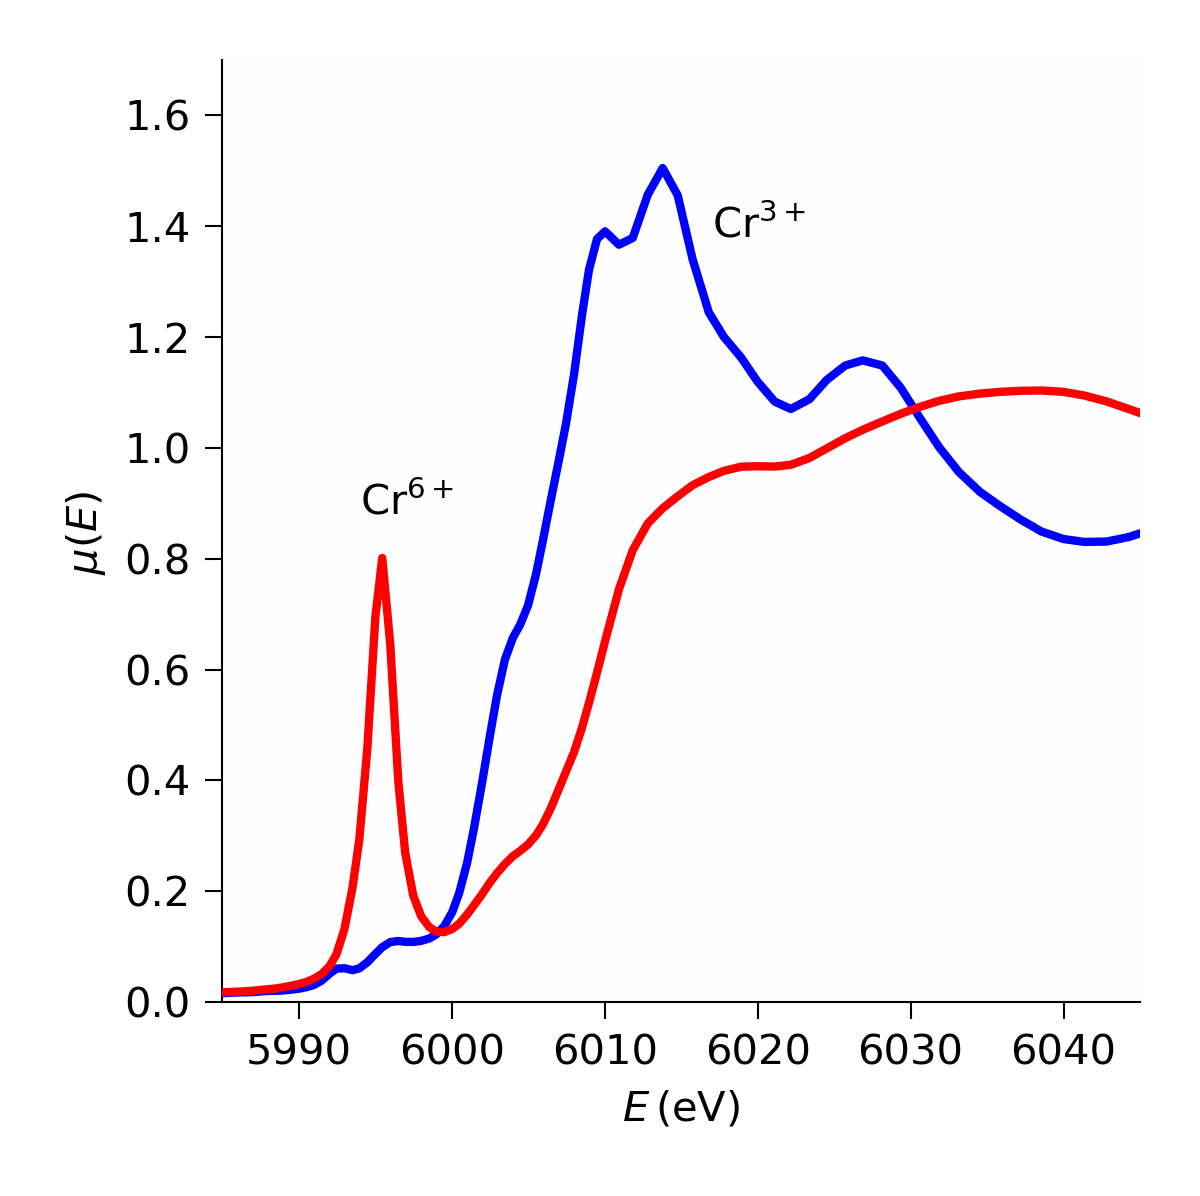
\includegraphics[width=52mm]{figs/xanes/cr}
    \end{minipage}
    &
    \onslide+<1->
    \begin{minipage}{55mm}
      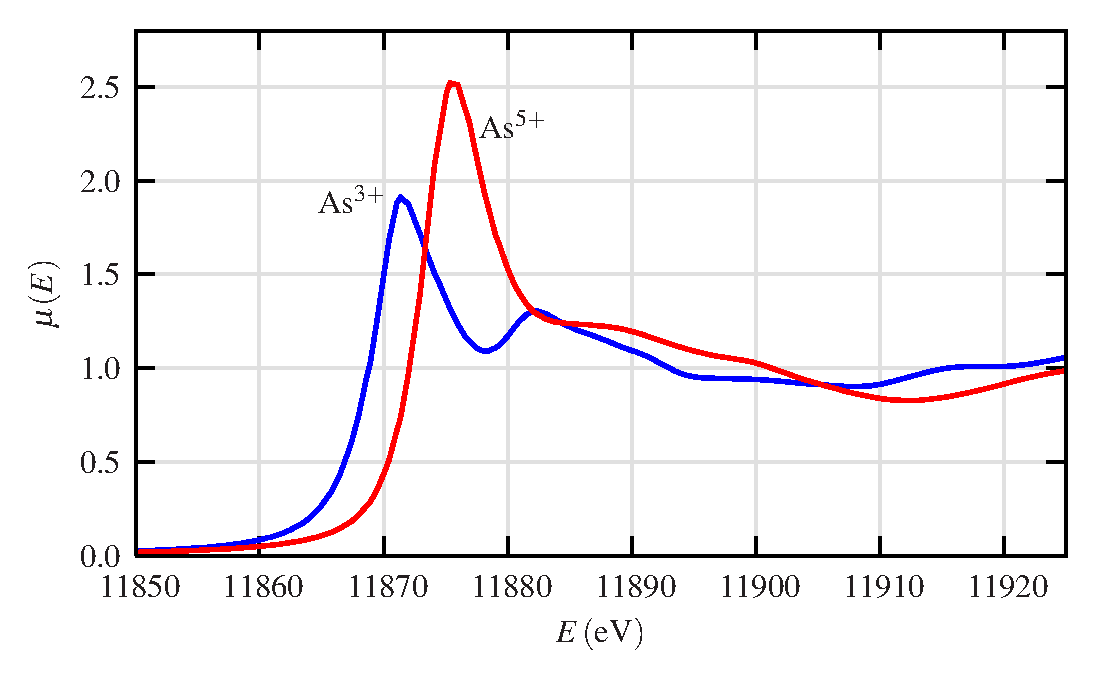
\includegraphics[width=52mm]{figs/xanes/as}
    \end{minipage} \\
    \onslide+<1->
    \hspace{3mm} Cr K-edge for $\rm Cr^{3+}$ and $\rm Cr^{6+}$
    &
    \onslide+<1->
    \hspace{3mm}   As K-edge for $\rm As^{3+}$ and $\rm As^{5+}$
  \end{tabular}

  \onslide+<2->{
    \begin{cenpage}{110mm}
      Analyzing XANES: \vmm

      \hspace{3mm} 1.  Linearly combine known spectra to match measured spectra.

      \vmm

      \hspace{3mm} 2. {\emph{ab initio}} calculations to map features
      to electronic density of states.
    \end{cenpage}
    }
\vfill
\end{slide}
